\chapter{Proposta do Sistema}
\label{cap:resultados}

Este capítulo apresenta a proposta detalhada de um mercado financeiro poupador baseado em blockchain como alternativa ao sistema previdenciário atual. A proposta é estruturada em cinco componentes principais: arquitetura geral, mecanismo de contribuição e investimento, sistema de governança, regras operacionais e mecanismos de herança.

\section{Visão Geral da Proposta}

O sistema proposto visa criar um mercado financeiro poupador que substitua gradualmente o INSS e o FGTS, permitindo que os trabalhadores brasileiros acumulem patrimônio próprio através de investimentos em empresas nacionais. A proposta combina elementos do modelo australiano de Superannuation com as capacidades da tecnologia blockchain para criar um sistema transparente, seguro e com governança compartilhada.

Os princípios fundamentais do sistema são:
\begin{alineas}
    \item \textbf{Propriedade individual}: Os recursos pertencem ao trabalhador, não ao Estado;
    \item \textbf{Investimento produtivo}: Os recursos são direcionados a empresas reais, gerando retorno econômico;
    \item \textbf{Governança compartilhada}: Controle dividido entre trabalhador e governo, evitando uso indevido;
    \item \textbf{Transparência nas regras}: Código auditável, com privacidade nas transações individuais;
    \item \textbf{Automatização}: Regras executadas por smart contracts, reduzindo burocracia.
\end{alineas}

\section{Arquitetura do Sistema}

A arquitetura proposta é composta por três camadas principais, conforme ilustrado na Figura \ref{fig:arquitetura}.

\begin{figure}[htb]
    \centering
    \caption{Arquitetura do Sistema Proposto}
    \label{fig:arquitetura}
    \begin{tikzpicture}[
        node distance=1.5cm,
        box/.style={rectangle, draw, minimum width=4cm, minimum height=1cm, align=center},
        arrow/.style={->, >=stealth, thick}
    ]
        % Camada de Usuário
        \node[box, fill=blue!20] (user) {Camada de Usuário\\(Interface Web/Mobile)};
        
        % Camada de Aplicação
        \node[box, fill=green!20, below=of user] (app) {Camada de Aplicação\\(Smart Contracts)};
        
        % Camada de Blockchain
        \node[box, fill=orange!20, below=of app] (chain) {Camada de Blockchain\\(Rede Distribuída)};
        
        % Conexões
        \draw[arrow] (user) -- (app);
        \draw[arrow] (app) -- (chain);
        
        % Atores externos
        \node[box, fill=gray!20, right=2cm of user] (trab) {Trabalhador};
        \node[box, fill=gray!20, right=2cm of app] (gov) {Governo};
        \node[box, fill=gray!20, right=2cm of chain] (emp) {Empresas};
        
        \draw[arrow] (trab) -- (user);
        \draw[arrow] (gov) -- (app);
        \draw[arrow] (emp) -- (chain);
    \end{tikzpicture}
    \fonte{LIMA (2026).}
\end{figure}

\subsection{Camada de Blockchain}

A camada base utiliza uma blockchain permissionada, operada por nós validadores distribuídos entre diferentes instituições (Banco Central, órgãos reguladores, grandes instituições financeiras). A escolha por blockchain permissionada, em vez de pública, justifica-se por:

\begin{alineas}
    \item Maior controle sobre quem pode validar transações;
    \item Melhor desempenho em termos de transações por segundo;
    \item Conformidade regulatória mais facilitada;
    \item Menor consumo energético comparado a redes de prova de trabalho.
\end{alineas}

\subsection{Camada de Smart Contracts}

Esta camada implementa toda a lógica de negócio do sistema através de smart contracts, incluindo:

\begin{alineas}
    \item \textbf{Contrato de Contribuição}: Recebe os depósitos mensais e registra na conta do trabalhador;
    \item \textbf{Contrato de Investimento}: Gerencia as ordens de compra e venda de ativos;
    \item \textbf{Contrato Multi-sig}: Implementa a governança compartilhada;
    \item \textbf{Contrato de Herança}: Gerencia a transferência de ativos em caso de falecimento;
    \item \textbf{Contrato de Compliance}: Verifica o cumprimento das regras operacionais.
\end{alineas}

\subsection{Camada de Usuário}

A interface de usuário consiste em aplicativo móvel e plataforma web que permitem ao trabalhador:

\begin{alineas}
    \item Visualizar seu saldo e histórico de contribuições;
    \item Consultar sua carteira de investimentos;
    \item Solicitar a operação mensal permitida;
    \item Acompanhar a rentabilidade de seus investimentos;
    \item Gerenciar beneficiários para herança.
\end{alineas}

\section{Mecanismo de Contribuição e Investimento}

\subsection{Fluxo de Contribuição}

O fluxo de contribuição proposto mantém a estrutura atual de desconto em folha, porém com destino diferente:

\begin{enumerate}
    \item O empregador desconta o percentual do salário do trabalhador (similar ao atual);
    \item O valor é convertido em tokens estáveis (stablecoins pareadas ao Real);
    \item Os tokens são depositados automaticamente na carteira multi-sig do trabalhador;
    \item O smart contract registra a transação e atualiza o saldo disponível para investimento.
\end{enumerate}

\subsection{Universo de Investimentos}
\label{sec:universo-investimentos}

O sistema propõe a criação de uma \textbf{bolsa tokenizada pareada em 1:1 com a B3}, onde cada ativo negociado na bolsa tradicional possui um token correspondente na blockchain previdenciária. Essa estrutura permite que os trabalhadores invistam nos mesmos ativos disponíveis no mercado convencional, porém com uma diferença fundamental: \textbf{privacidade de propriedade}.

Diferentemente do sistema tradicional, onde a CVM, corretoras e diversos intermediários têm acesso à identidade dos acionistas, os tokens previdenciários são projetados para que \textbf{apenas o próprio titular conheça sua carteira de investimentos}. A blockchain registra a existência e validade dos tokens, mas a vinculação entre endereço da carteira e identidade do trabalhador permanece criptograficamente protegida. Essa arquitetura:

\begin{alineas}
    \item Impede que governos futuros identifiquem e tributem seletivamente determinados perfis de investidores;
    \item Protege o trabalhador contra perseguições políticas baseadas em suas escolhas de investimento;
    \item Elimina o risco de ``caça às bruxas'' contra quem investiu em setores posteriormente considerados controversos;
    \item Preserva a fungibilidade dos tokens, já que não carregam histórico de propriedade rastreável.
\end{alineas}

Os recursos podem ser investidos exclusivamente em ativos de empresas brasileiras, incluindo:

\begin{alineas}
    \item Ações de empresas listadas na B3;
    \item Debêntures de empresas brasileiras;
    \item Fundos de investimento em infraestrutura (FI-Infra);
    \item Fundos imobiliários (FIIs);
    \item Títulos públicos federais (como opção conservadora).
\end{alineas}

A restrição a ativos nacionais tem como objetivo:
\begin{alineas}
    \item Fomentar o mercado de capitais brasileiro;
    \item Financiar o crescimento de empresas nacionais;
    \item Evitar a evasão de divisas;
    \item Criar um ciclo virtuoso de poupança e investimento interno.
\end{alineas}

\subsection{Tokenização de Ativos}

Os ativos elegíveis seriam tokenizados, ou seja, representados por tokens na blockchain. Cada token representa uma fração do ativo subjacente, permitindo:

\begin{alineas}
    \item Investimentos fracionados, acessíveis a pequenos poupadores;
    \item Liquidação instantânea de operações;
    \item Registro imutável de propriedade;
    \item Auditabilidade completa das transações.
\end{alineas}

\section{Sistema de Governança Multi-sig}

O elemento central da proposta é o sistema de governança baseado em carteiras multi-assinatura, que implementa o controle compartilhado entre trabalhador e governo.

\subsection{Estrutura das Chaves}

Cada carteira previdenciária opera com um esquema 2-de-2, onde ambas as chaves são necessárias para autorizar transações:

\begin{alineas}
    \item \textbf{Chave do Trabalhador}: Controlada exclusivamente pelo titular da conta, armazenada em dispositivo pessoal seguro;
    \item \textbf{Chave do Governo}: Controlada por órgão regulador (ex: Banco Central ou nova autarquia), utilizada para co-assinar transações válidas.
\end{alineas}

\subsection{Fluxo de Autorização}

Para realizar qualquer movimentação, o seguinte fluxo é executado:

\begin{enumerate}
    \item O trabalhador inicia a solicitação através do aplicativo, assinando com sua chave;
    \item O smart contract verifica se a operação está dentro das regras permitidas;
    \item Se válida, a solicitação é encaminhada ao sistema governamental;
    \item O sistema governamental co-assina automaticamente se todas as regras forem cumpridas;
    \item A transação é executada e registrada na blockchain.
\end{enumerate}

Este modelo garante que:
\begin{alineas}
    \item O governo sozinho não pode mover os recursos do trabalhador;
    \item O trabalhador sozinho não pode violar as regras do sistema;
    \item Há transparência nas regras, preservando a privacidade individual das transações.
\end{alineas}

\subsection{Diagrama do Sistema Multi-sig}

A Figura \ref{fig:multisig} ilustra o funcionamento do sistema de governança multi-sig.

\begin{figure}[htb]
    \centering
    \caption{Sistema de Governança Multi-sig}
    \label{fig:multisig}
    \begin{tikzpicture}[
        node distance=2cm,
        key/.style={circle, draw, minimum size=1.5cm, align=center, fill=yellow!30},
        wallet/.style={rectangle, draw, minimum width=3cm, minimum height=2cm, align=center, fill=green!20},
        arrow/.style={->, >=stealth, thick}
    ]
        % Carteira central
        \node[wallet] (wallet) {Carteira\\Multi-sig\\(2 de 2)};
        
        % Chaves
        \node[key, above left=of wallet] (key1) {Chave\\Trabalhador};
        \node[key, above right=of wallet] (key2) {Chave\\Governo};
        
        % Conexões
        \draw[arrow] (key1) -- (wallet);
        \draw[arrow] (key2) -- (wallet);
    \end{tikzpicture}
    \fonte{LIMA (2026).}
\end{figure}

\section{Regras Operacionais}

Para garantir que o sistema cumpra seu objetivo previdenciário, são impostas regras operacionais rígidas, implementadas diretamente nos smart contracts.

\subsection{Restrição de Operações}

Cada trabalhador pode realizar no máximo um lote de operações de compra e venda por mês. Esta restrição visa:

\begin{alineas}
    \item Evitar comportamento especulativo de curto prazo;
    \item Incentivar visão de longo prazo nos investimentos;
    \item Reduzir custos operacionais e de processamento;
    \item Simplificar a gestão da carteira pelo trabalhador médio.
\end{alineas}

\subsection{Bloqueio de Liquidação}

Os recursos são bloqueados até a aposentadoria, com exceções limitadas:

\begin{alineas}
    \item Aposentadoria por idade ou tempo de contribuição;
    \item Invalidez permanente comprovada;
    \item Doenças graves especificadas em lei;
    \item Falecimento (transferência para herdeiros).
\end{alineas}

Diferentemente do FGTS atual, não há saque para compra de imóvel ou demissão, reforçando o caráter estritamente previdenciário dos recursos.

\subsection{Operações}

As contribuições mensais do trabalhador são depositadas inicialmente na forma de \textbf{stablecoin pareada ao Real} (token BRL), representando saldo disponível para investimento. A partir do primeiro mês de contribuição, o trabalhador pode converter esses tokens em \textbf{ativos tokenizados} --- ações, debêntures, fundos imobiliários e demais ativos elegíveis conforme descrito na Seção \ref{sec:universo-investimentos}.

Uma vez investidos, os ativos geram rendimentos conforme sua natureza: dividendos de ações, juros de debêntures, aluguéis de FIIs, entre outros. Esses \textbf{dividendos são creditados mensalmente} na carteira do trabalhador, também na forma de tokens BRL. Contudo, diferentemente do saldo principal, os dividendos \textbf{não são sacáveis} --- permanecem sujeitos às mesmas regras de bloqueio até a aposentadoria.

A utilidade imediata dos dividendos está no \textbf{reinvestimento}: o trabalhador pode, dentro do lote mensal de operações permitido, converter os dividendos recebidos em novos ativos tokenizados. Este mecanismo cria um ciclo virtuoso de capitalização composta:

\begin{alineas}
    \item \textbf{Mês 1}: Contribuição inicial convertida em ativos;
    \item \textbf{Mês 2 em diante}: Contribuição + dividendos do mês anterior disponíveis para reinvestimento;
    \item \textbf{Efeito acumulativo}: Os dividendos reinvestidos geram novos dividendos, acelerando o crescimento patrimonial.
\end{alineas}

Esta arquitetura incentiva o trabalhador a manter seus recursos investidos em ativos produtivos, maximizando o potencial de crescimento de longo prazo enquanto mantém a disciplina previdenciária de não permitir saques antecipados.

\subsection{Limites de Concentração}

Para proteção do trabalhador, o sistema oferece limites de diversificação configuráveis. Os valores específicos --- como percentual máximo por empresa ou por setor --- podem ser definidos de forma flexível no momento da adesão. Contudo, uma vez escolhidos e aceitos pelo trabalhador, esses limites tornam-se \textbf{imutáveis} para aquela carteira, garantindo que regras não sejam alteradas retroativamente em prejuízo do titular.

Alternativamente, o sistema pode oferecer \textbf{atualizações opcionais} de regras: quando novos limites forem propostos pelo órgão regulador, o trabalhador recebe notificação e decide se aceita ou não a mudança. Caso recuse, sua carteira continua operando sob as regras originalmente contratadas. Exemplos de limites configuráveis:

\begin{alineas}
    \item Percentual máximo do patrimônio em uma única empresa;
    \item Percentual máximo em um único setor da economia;
    \item Percentual mínimo em ativos de baixo risco (títulos públicos ou equivalentes).
\end{alineas}

Essa arquitetura preserva a autonomia do trabalhador enquanto impede que governos futuros imponham unilateralmente restrições prejudiciais aos investimentos já realizados.

\subsection{Tabela de Regras Operacionais}

A Tabela \ref{tab:regras} resume as principais regras operacionais do sistema.

\begin{table}[htb]
    \centering
    \caption{Resumo das Regras Operacionais}
    \label{tab:regras}
    \begin{tabular}{p{5cm}p{8cm}}
        \toprule
        \textbf{Regra} & \textbf{Descrição} \\
        \midrule
        Operações mensais & Máximo 1 lote de compra/venda por mês \\
        Ativos elegíveis & Apenas empresas/ativos brasileiros \\
        Limites de concentração & Configuráveis na adesão, imutáveis após aceite \\
        Saque & Apenas na aposentadoria ou exceções legais \\
        Governança & Multi-sig 2-de-2 (trabalhador + governo) \\
        \bottomrule
    \end{tabular}
    \fonte{LIMA (2026).}
\end{table}

\section{Mecanismo de Herança}

Um diferencial importante do sistema proposto é o tratamento da herança, que difere fundamentalmente do INSS atual.

\subsection{Herança Total do Patrimônio}

No sistema proposto, em caso de falecimento do titular, 100\% do patrimônio acumulado é transferido para os herdeiros designados. Isso contrasta com o sistema atual, onde o trabalhador que falece antes de se aposentar perde grande parte de suas contribuições.

Um princípio fundamental desta proposta é que \textbf{o governo não deve ter gerência sobre como os ganhos do trabalhador serão usufruídos após sua morte}. Diferentemente do direito sucessório tradicional, que impõe regras de parentesco e quotas obrigatórias, o sistema previdenciário proposto confere ao titular \textbf{autonomia absoluta} na designação de seus beneficiários. O trabalhador pode escolher livremente quem receberá seu patrimônio --- sejam familiares, amigos, instituições ou qualquer pessoa de sua confiança --- assumindo integralmente o risco de suas escolhas.

É importante ressaltar que esse nível de autonomia patrimonial \textbf{já existe para os mais ricos}, através de estruturas jurídicas sofisticadas como \textit{holdings} familiares, \textit{trusts} internacionais e fundações privadas. Esses instrumentos permitem às elites econômicas contornar as regras de sucessão obrigatória, proteger patrimônio de credores e designar livremente seus beneficiários. Contudo, os custos de implementação e manutenção dessas estruturas --- honorários advocatícios, taxas de constituição, contabilidade especializada e consultoria tributária --- frequentemente superam o patrimônio total acumulado por um trabalhador médio ao longo de toda sua vida. O sistema proposto \textbf{democratiza esse direito}, conferindo ao trabalhador comum as mesmas garantias patrimoniais hoje restritas às elites, sem custos adicionais além da própria contribuição previdenciária.

Esta abordagem confere autonomia absoluta ao trabalhador na designação de seus beneficiários, permitindo que apenas aqueles expressamente designados --- e que possuam a chave privada compartilhada em vida --- tenham acesso ao patrimônio, eliminando heranças indesejadas decorrentes de vínculos legais que não refletem a real vontade do titular.

O trabalhador pode, a qualquer momento, cadastrar seus beneficiários no sistema, especificando:

\begin{alineas}
    \item Endereço da carteira do sucessor;
    \item Percentual destinado a cada beneficiário.
\end{alineas}

\subsection{Processo de Transferência}

Em caso de falecimento:

\begin{enumerate}
    \item A família apresenta certidão de óbito e a chave privada do titular falecido;
    \item O patrimônio é transferido para novas carteiras multi-sig dos herdeiros;
    \item Os herdeiros assumem o controle, mantendo as mesmas regras operacionais;
    \item Os recursos permanecem bloqueados até que cada herdeiro atinja sua própria idade de aposentadoria.
\end{enumerate}

Esta regra de bloqueio até a aposentadoria do herdeiro garante o incentivo à produção e à necessidade do trabalho ao longo de toda a vida, evitando que heranças previdenciárias se tornem mecanismo de ociosidade.

\section{Transição do Sistema Atual}

A implementação do sistema proposto requer o pagamento integral da dívida previdenciária acumulada antes da migração completa. Esta premissa é inegociável: nenhum trabalhador deve ser prejudicado pela transição.

\subsection{Estratégia de Transição Gradual}

A migração inicia obrigatoriamente pelos \textbf{trabalhadores mais jovens}, ordenados por ano de nascimento. Esta escolha é estratégica: os cidadãos mais novos acumularam relativamente poucas contribuições ao sistema atual, resultando em valores de quitação significativamente menores. Um trabalhador de 20 anos pode ter contribuído por apenas 2-3 anos, enquanto um de 55 anos acumula décadas de contribuições que precisam ser reconhecidas e pagas.

Simultaneamente, o governo deve iniciar o pagamento aos \textbf{trabalhadores mais velhos}, demonstrando seu comprometimento genuíno com a transição. Contudo, há uma diferença fundamental no cálculo da dívida para esta faixa etária: \textbf{os idosos já receberam boa parte do que aportaram em vida}. Um aposentado de 80 anos que contribuiu por 35 anos e já recebe benefícios há 15 anos teve grande parte de suas contribuições retornadas na forma de aposentadoria mensal. O saldo devedor, portanto, é substancialmente menor do que o valor bruto contribuído --- podendo inclusive ser negativo para aqueles que já receberam mais do que aportaram.

Esta realidade altera significativamente a dinâmica de custos da transição. Enquanto os jovens possuem valores individuais baixos mas são numerosos, os idosos possuem valores individuais potencialmente baixos (ou nulos) e são menos numerosos. O resultado é que, com a mesma dotação orçamentária, a frente jovem avança mais lentamente em termos de faixas etárias cobertas, enquanto a frente sênior pode cobrir rapidamente as idades mais avançadas.

Esta abordagem bidirecional --- jovens e idosos sendo atendidos em paralelo --- cria um efeito pedagógico importante: assim como na transição tecnológica digital, onde os jovens frequentemente ensinam os mais velhos a utilizar novas ferramentas, espera-se que a familiaridade dos jovens com o novo sistema facilite a adoção pelos mais experientes.

As \textbf{velocidades de migração} devem ser proporcionais à capacidade de pagamento. Propõe-se alocar metade do valor disponível em caixa para cada frente:

\begin{alineas}
    \item \textbf{50\% para a frente jovem}: Cobre poucas faixas etárias por período, pois há muitas pessoas com valores baixos cada;
    \item \textbf{50\% para a frente sênior}: Cobre muitas faixas etárias rapidamente, pois há poucas pessoas com saldo devedor reduzido.
\end{alineas}

Esta estratégia bidirecional apresenta vantagens significativas:

\begin{alineas}
    \item \textbf{Sinalização política}: O pagamento aos sêniores demonstra que não se trata de calote geracional;
    \item \textbf{Transferência de conhecimento}: Os jovens, nativos digitais, auxiliam os mais velhos na adaptação ao novo sistema;
    \item \textbf{Convergência gradual}: As duas frentes eventualmente se encontram na faixa etária intermediária (40-50 anos), onde estão os maiores saldos devedores.
\end{alineas}

A Figura \ref{fig:transicao-geracional} ilustra a dinâmica da transição, mostrando a relação entre idade e valor \textit{líquido} devido --- ou seja, contribuições menos benefícios já recebidos.

\begin{figure}[htb]
    \centering
    \caption{Estratégia de Transição Bidirecional por Faixa Etária}
    \label{fig:transicao-geracional}
    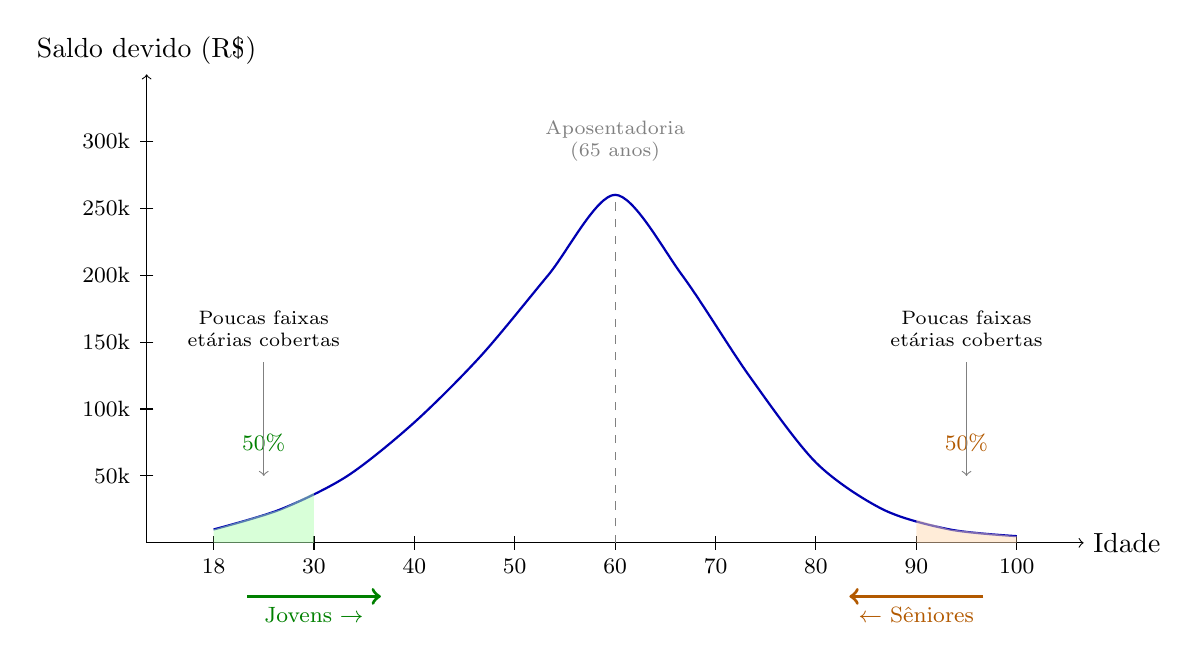
\begin{tikzpicture}[scale=0.85]
        % Eixos
        \draw[->] (0,0) -- (14,0) node[right] {Idade};
        \draw[->] (0,0) -- (0,7) node[above] {Saldo devido (R\$)};
        
        % Labels do eixo X
        \foreach \x/\label in {1/18, 2.5/30, 4/40, 5.5/50, 7/60, 8.5/70, 10/80, 11.5/90, 13/100} {
            \draw (\x,0.1) -- (\x,-0.1) node[below] {\footnotesize \label};
        }
        
        % Labels do eixo Y
        \foreach \y/\label in {1/50k, 2/100k, 3/150k, 4/200k, 5/250k, 6/300k} {
            \draw (0.1,\y) -- (-0.1,\y) node[left] {\footnotesize \label};
        }
        
        % Curva de saldo devido (cresce até aposentadoria, depois cai rapidamente com benefícios recebidos)
        \draw[thick, blue!70!black] plot[smooth] coordinates {
            (1, 0.2) (2, 0.5) (3, 1.0) (4, 1.8) (5, 2.8) (6, 4.0) (7, 5.2) (8, 4.0) (9, 2.5) (10, 1.2) (11, 0.5) (12, 0.2) (13, 0.1)
        };
        
        % Área de migração jovens (50% do orçamento - área pequena pois valores baixos por pessoa)
        \fill[green!30, opacity=0.5] (1,0) -- (1,0.2) -- (2,0.5) -- (2.5,0.75) -- (2.5,0) -- cycle;
        \node[green!50!black, font=\footnotesize, align=center] at (1.75, 1.5) {50\%};
        
        % Área de migração sêniores (50% do orçamento - área igual pois valores baixos por pessoa)
        \fill[orange!30, opacity=0.5] (11.5,0) -- (11.5,0.35) -- (12,0.2) -- (13,0.1) -- (13,0) -- cycle;
        \node[orange!70!black, font=\footnotesize, align=center] at (12.25, 1.5) {50\%};
        
        % Linha vertical indicando idade de aposentadoria
        \draw[dashed, gray] (7, 0) -- (7, 5.2);
        \node[gray, font=\scriptsize, align=center] at (7, 6.0) {Aposentadoria\\(65 anos)};
        
        % Setas indicando direção da migração
        \draw[->, very thick, green!50!black] (1.5, -0.8) -- (3.5, -0.8) node[midway, below] {\footnotesize Jovens $\rightarrow$};
        \draw[->, very thick, orange!70!black] (12.5, -0.8) -- (10.5, -0.8) node[midway, below] {\footnotesize $\leftarrow$ Sêniores};
        
        % Anotações explicativas
        \node[font=\scriptsize, align=center, text width=2.5cm] at (1.75, 3.2) {Poucas faixas\\etárias cobertas};
        \draw[->, gray, thin] (1.75, 2.7) -- (1.75, 1.0);
        
        \node[font=\scriptsize, align=center, text width=2.5cm] at (12.25, 3.2) {Poucas faixas\\etárias cobertas};
        \draw[->, gray, thin] (12.25, 2.7) -- (12.25, 1.0);
    \end{tikzpicture}
    \fonte{LIMA (2026), com base em dados do Anuário Estatístico da Previdência Social \cite{aeps2023}.}
\end{figure}

\subsection{Financiamento da Transição}

O principal desafio da transição é o financiamento dos benefícios atuais enquanto as contribuições são direcionadas ao novo sistema. Propõe-se:

\begin{alineas}
    \item Utilização de receitas do patrimônio público (royalties, dividendos de estatais);
    \item Recursos provenientes do arrendamento do patrimônio nacional conforme proposto na Seção \ref{cap:fundamentacao-teorica};
    \item Redução gradual do déficit primário através de reformas administrativas;
    \item Emissão de títulos de longo prazo específicos para a transição previdenciária.
\end{alineas}

\section{Benefícios Esperados}

A implementação do sistema proposto traria benefícios em múltiplas dimensões:

\subsection{Para o Trabalhador}

\begin{alineas}
    \item Propriedade real sobre os recursos poupados;
    \item Rentabilidade potencialmente superior à inflação;
    \item Herança garantida para a família;
    \item Transparência nas regras, com privacidade sobre saldos individuais;
    \item Segurança jurídica equivalente à que hoje leva pessoas a investirem em criptomoedas e mercado de capitais internacional.
\end{alineas}

\subsection{Para a Economia}

\begin{alineas}
    \item Aumento da taxa de poupança nacional;
    \item Desenvolvimento do mercado de capitais;
    \item Redução do custo de capital para empresas;
    \item Financiamento de investimentos produtivos;
    \item Diminuição da evasão de capital para offshores.
\end{alineas}

\subsection{Para o Estado}

\begin{alineas}
    \item Eliminação gradual do déficit previdenciário;
    \item Liberação de recursos para investimentos públicos;
    \item Redução da carga tributária potencial no longo prazo;
    \item Modernização da infraestrutura financeira.
\end{alineas}

\section{Desafios e Riscos}

A proposta também apresenta desafios significativos:

\subsection{Desafios Técnicos}

\begin{alineas}
    \item Escalabilidade da blockchain para milhões de usuários;
    \item Segurança cibernética e proteção das chaves privadas;
    \item Integração com sistemas legados e bases governamentais;
    \item Educação financeira da população.
\end{alineas}

\subsection{Desafios Políticos}

\begin{alineas}
    \item Resistência de grupos beneficiados pelo sistema atual;
    \item Necessidade de reforma constitucional;
    \item Coordenação entre múltiplos órgãos governamentais;
    \item Comunicação efetiva com a população.
\end{alineas}

\subsection{Riscos de Mercado}

\begin{alineas}
    \item Exposição dos trabalhadores a volatilidade do mercado;
    \item Possibilidade de perdas em períodos de crise;
    \item Necessidade de mecanismos de proteção para trabalhadores próximos à aposentadoria.
\end{alineas}

\section{Arquitetura do Mercado em Blockchain Permissionada}

Esta seção detalha como o mercado financeiro poupador pode ser implementado utilizando uma blockchain permissionada, onde os nós validadores são operados por entidades autorizadas (governo, instituições financeiras reguladas), garantindo transparência, segurança e conformidade regulatória.

\subsection{Camadas da Arquitetura}

O sistema é organizado em cinco camadas interdependentes, conforme ilustrado na Figura \ref{fig:camadas-mercado}.

\begin{figure}[htb]
    \centering
    \caption{Arquitetura em Camadas do Mercado}
    \label{fig:camadas-mercado}
    \begin{tikzpicture}[
        node distance=0.8cm,
        layer/.style={rectangle, draw, minimum width=12cm, minimum height=1.2cm, align=center, font=\small}
    ]
        \node[layer, fill=blue!15] (l1) {Camada de Interface};
        \node[layer, fill=green!15, below=of l1] (l2) {Camada de Governança};
        \node[layer, fill=yellow!15, below=of l2] (l3) {Camada de Mercado};
        \node[layer, fill=orange!15, below=of l3] (l4) {Camada de Tokenização};
        \node[layer, fill=red!15, below=of l4] (l5) {Camada de Oracle};
    \end{tikzpicture}
    \fonte{LIMA (2026).}
\end{figure}

\subsubsection{Camada de Interface}

A camada de interface é o ponto de contato entre o usuário e o sistema previdenciário. Através de aplicações web (dApps) ou aplicativos móveis, o trabalhador pode visualizar seu saldo, executar operações de compra e venda de ativos, gerenciar beneficiários e acompanhar o desempenho de sua carteira. A interface abstrai a complexidade da blockchain, oferecendo uma experiência similar aos aplicativos bancários tradicionais.

\subsubsection{Camada de Governança}

A camada de governança implementa o modelo multi-sig descrito anteriormente, onde as regras de controle compartilhado entre indivíduo e governo são codificadas. Esta camada é responsável por validar permissões, verificar condições (como idade para liquidação) e garantir que nenhuma parte possa agir unilateralmente fora das regras estabelecidas.

\subsubsection{Camada de Mercado}

A camada de mercado é responsável pela execução das operações de compra e venda de ativos tokenizados. Pode ser implementada através de livros de ordens descentralizados, onde compradores e vendedores postam ordens que são casadas automaticamente, ou através de formadores de mercado automatizados que garantem liquidez constante.

\subsubsection{Camada de Tokenização}

A tokenização de ativos reais é o fundamento do mercado descentralizado. Cada ação negociada na B3 é representada por um token na blockchain, mantendo paridade 1:1 com o ativo custodiado:

\begin{alineas}
    \item \textbf{Custódia Regulada}: Instituição custodiante autorizada pela CVM mantém as ações reais na CBLC (Companhia Brasileira de Liquidação e Custódia);
    \item \textbf{\textit{Circuit Breaker}}: Mecanismo de emergência para pausar operações em caso de inconsistências.
\end{alineas}

\subsubsection{Camada de Oracle}

Os oracles são responsáveis por sincronizar informações do mundo real com a blockchain. Utilizam dados oficiais da B3 como fonte autoritativa de preços, com \textit{heartbeat} (atualizações periódicas obrigatórias) durante o pregão e pausa automática sincronizada com o \textit{circuit breaker} da B3.

\subsection{Poderes do Smart Contract Multi-Sig}

O elemento central da governança é a definição precisa dos poderes de cada parte. A Tabela \ref{tab:poderes-multisig} apresenta a matriz de poderes implementada no smart contract.

\begin{table}[htb]
    \centering
    \caption{Matriz de Poderes do Smart Contract Multi-Sig}
    \label{tab:poderes-multisig}
    \begin{tabular}{p{4cm}ccp{4cm}}
        \toprule
        \textbf{Operação} & \textbf{Indivíduo} & \textbf{Governo} & \textbf{Condição} \\
        \midrule
        Trade mensal & \checkmark Exclusivo & $\times$ Bloqueado & Cooldown 30 dias \\
        Liquidação total & $\times$ Bloqueado & $\times$ Bloqueado & Idade $<$ 65 anos \\
        Liquidação total & \checkmark Livre & -- N/A & Idade $\geq$ 65 anos \\
        Adicionar herdeiro & \checkmark Exclusivo & $\times$ Bloqueado & Sempre \\
        Distribuir herança & c/ Chave Primária & \checkmark Autoriza & Após óbito \\
        Liquidar estate & -- N/A & \checkmark Pleno & Após 100 anos \\
        Whitelist de ativos & $\times$ Bloqueado & \checkmark Exclusivo & Sempre \\
        \bottomrule
    \end{tabular}
    \fonte{LIMA (2026).}
\end{table}

\subsubsection{Poderes do Indivíduo}

O indivíduo (trabalhador) possui os seguintes poderes exclusivos:

\begin{alineas}
    \item \textbf{Executar Trades}: Pode comprar e vender ativos livremente dentro do universo de investimentos permitido, respeitando o limite de 1 operação por mês;
    \item \textbf{Gerenciar Beneficiários}: Tem controle exclusivo sobre quem são seus herdeiros e qual percentual cada um receberá;
    \item \textbf{Prova de Vida}: Deve submeter prova de vida anual para manter sua carteira ativa;
    \item \textbf{Plenos Poderes após 65 anos}: Ao atingir a idade de aposentadoria, pode liquidar qualquer posição sem necessidade de aprovação governamental.
\end{alineas}

É fundamental notar que o governo \textbf{não pode} fazer trades em nome do indivíduo. Esta restrição garante que a alocação de capital seja feita pela ``mão invisível'' das decisões individuais agregadas, não por uma autoridade central.

\subsubsection{Poderes do Governo}

O governo possui poderes específicos e limitados:

\begin{alineas}
    \item \textbf{Whitelist de Ativos}: Controla quais ativos podem ser negociados no sistema, garantindo que apenas empresas brasileiras reguladas participem;
    \item \textbf{Distribuição de Herança}: Autoriza a transferência de ativos para os beneficiários cadastrados, apenas em caso de óbito e mediante posse da chave primária pela família;
    \item \textbf{Plenos Poderes após 100 anos}: Em caso de ausência de prova de vida por 100 anos, assume controle total para liquidação do estate.
\end{alineas}

\subsubsection{Checks and Balances}

O sistema implementa um mecanismo de freios e contrapesos onde:

\begin{alineas}
    \item O indivíduo sozinho não pode liquidar antes dos 65 anos (protege contra gastos impulsivos);
    \item O governo sozinho não pode mover os ativos (protege contra confisco arbitrário);
    \item O código é imutável após deploy (protege contra mudanças políticas);
    \item O código é público e auditável (garante transparência das regras, não dos saldos individuais).
\end{alineas}

\subsection{Descentralização Progressiva}

A implementação do sistema pode seguir um caminho de descentralização progressiva:

\textbf{Fase 1 - Federada (Anos 1-5):} Governo opera os nós validadores, custodiantes regulados pela CVM, contratos auditados mas upgradáveis via timelock.

\textbf{Fase 2 - Híbrida (Anos 6-15):} Validadores distribuídos (40\% governo, 60\% entidades privadas), DAO para propostas de mudança, contratos com timelock de 30 dias para upgrades.

\textbf{Fase 3 - Descentralizada (Anos 16+):} Validadores eleitos por stake, governança 100\% on-chain, contratos imutáveis.

\section{O Problema do Bloqueio}

Historicamente, governos exercem pressão sobre a segurança jurídica dos indivíduos e buscam controlar o valor de seus bens. Na criação do Bitcoin, Satoshi Nakamoto incluiu a seguinte mensagem no bloco gênesis \cite{genesisblock2009}:

\begin{quote}
    \textit{``The Times 03/Jan/2009 Chancellor on brink of second bailout for banks''}
\end{quote}

Essa referência à manchete do jornal \textit{The Times} sobre o segundo resgate governamental aos bancos britânicos evidencia a predileção estatal pelas grandes elites financeiras, fenômeno amplamente documentado por Frédéric Bastiat em sua obra \textit{A Lei} (1850) \cite{bastiat1850}, onde o autor francês argumenta:

\begin{quote}
    \textit{``A lei pervertida! E os poderes de polícia do Estado pervertidos junto com ela! A lei, digo eu, não apenas desviada de seu propósito adequado, mas transformada para seguir um propósito inteiramente contrário! [...] A lei convertida em instrumento de espoliação!''}
\end{quote}

Portanto, deve haver uma maneira de o cidadão comum --- que não usufrui da mesma proteção jurídica aplicada a poucos --- obter algum benefício ao aportar em sua previdência sem correr risco de confisco.

\subsection{O Risco do Bloqueio de Ativos}

Para que o sistema funcione, os ativos de um indivíduo devem ser auditáveis: ele precisa ter acesso real aos tokens e o direito de trocá-los. Contudo, surge um problema crítico: se o governo conseguir vincular determinado token a determinado indivíduo, basta ordenar que todas as entidades financeiras sob sua jurisdição bloqueiem aquele token específico. Isso invalidaria completamente a proposta de segurança via blockchain.

O caso da China com o Bitcoin ilustra essa vulnerabilidade \cite{china2021}. O governo chinês não perseguiu diretamente os detentores de criptomoedas --- foi atrás das \textit{exchanges} centralizadas, que serviam como pontos de entrada e saída do ecossistema. Ao pressionar esses intermediários, conseguiu restringir significativamente o uso de Bitcoin no país sem precisar identificar cada usuário individualmente.

\subsection{Inviabilidade Prática do Bloqueio Massivo}

Para identificar e bloquear os ativos de um único indivíduo em um sistema com privacidade robusta, o governo precisaria dissolver todo o mecanismo de anonimização --- forçando \textbf{todos} os participantes a revelarem suas identidades e converterem seus tokens para ativos rastreáveis.

Para ilustrar a inviabilidade dessa abordagem, considere o seguinte cenário hipotético:

A \textbf{Klabin S.A.} (KLBN11), maior produtora e exportadora de papéis do Brasil, possui aproximadamente \textbf{1,1 milhão de acionistas pessoas físicas} registrados na B3 (dados de 2023). Se apenas \textbf{30\% desses acionistas} participassem do sistema previdenciário proposto, teríamos cerca de \textbf{330 mil indivíduos} cujos ativos estariam protegidos por anonimização.

Para bloquear os tokens de \textbf{um único suspeito}, o governo precisaria:

\begin{enumerate}
    \item Ordenar que todos os 330 mil participantes revelem suas identidades;
    \item Suspender temporariamente a negociação de todos os tokens vinculados à Klabin;
    \item Reemitir tokens rastreáveis após identificação completa;
    \item Reintegrar os participantes legítimos ao sistema.
\end{enumerate}

O custo operacional, jurídico e político de tal operação seria astronomicamente superior ao benefício de identificar um indivíduo. Multiplique esse cenário pelas \textbf{400+ empresas listadas na B3} e a impossibilidade prática torna-se evidente: o sistema seria autoimune a bloqueios cirúrgicos, protegendo o trabalhador comum sem impedir investigações legítimas em larga escala.

\subsubsection{Custo Financeiro de Bloqueio em Escala Nacional}

Para dimensionar a inviabilidade econômica de bloqueios massivos, considere os custos operacionais envolvidos. O Brasil possui aproximadamente \textbf{110 milhões de pessoas economicamente ativas} (PNAD 2023). Se todas participassem do sistema proposto:

\begin{table}[htb]
    \centering
    \caption{Custo Estimado de Bloqueio em Escala Nacional}
    \label{tab:custo-bloqueio}
    \begin{tabular}{p{6cm}c}
        \toprule
        \textbf{Métrica} & \textbf{Valor} \\
        \midrule
        População economicamente ativa & 110 milhões \\
        Custo de bloqueio por pessoa & R\$ 250-400 \\
        \textbf{Custo total para dissolução do sistema} & \textbf{R\$ 27,5 - 44 bilhões} \\
        Tempo estimado de processamento & 5-10 anos \\
        Processos judiciais gerados & $\sim$30-50 milhões \\
        \bottomrule
    \end{tabular}
    \fonte{LIMA (2026).}
\end{table}

Essa assimetria de custos cria uma \textbf{barreira econômica natural} contra abusos estatais: perseguir um indivíduo exigiria atacar milhões.

\subsection{A Solução da Monero: Privacidade por Design}

Criptomoedas como \textbf{Monero (XMR)} demonstram que a anonimização é tecnicamente viável \cite{monero2023}. A Monero utiliza três mecanismos principais para desvincular tokens de indivíduos:

\subsubsection{Ring Signatures (Assinaturas em Anel)}

Cada transação mistura a assinatura do remetente com outras assinaturas aleatórias, tornando impossível identificar quem realmente enviou os fundos. O remetente real é ``escondido'' entre múltiplos participantes fictícios, conforme ilustrado na Figura \ref{fig:ring-signatures}.

\begin{figure}[htb]
    \centering
    \caption{Funcionamento das Ring Signatures}
    \label{fig:ring-signatures}
    \begin{tikzpicture}[
        node distance=1.2cm,
        user/.style={circle, draw, minimum size=1cm, fill=gray!20},
        realuser/.style={circle, draw, minimum size=1cm, fill=green!40},
        tx/.style={rectangle, draw, minimum width=2.5cm, minimum height=1cm, fill=blue!20},
        arrow/.style={->, >=stealth, thick}
    ]
        % Usuários do anel
        \node[user] (u1) {A};
        \node[user, right=of u1] (u2) {B};
        \node[realuser, right=of u2] (u3) {C};
        \node[user, right=of u3] (u4) {D};
        \node[user, right=of u4] (u5) {E};
        
        % Transação
        \node[tx, below=2cm of u3] (tx) {Transação};
        
        % Conexões
        \draw[arrow, dashed] (u1) -- (tx);
        \draw[arrow, dashed] (u2) -- (tx);
        \draw[arrow, thick, green!60!black] (u3) -- (tx);
        \draw[arrow, dashed] (u4) -- (tx);
        \draw[arrow, dashed] (u5) -- (tx);
        
        % Legenda
        \node[below=0.5cm of tx, align=center] {\small Observador não consegue distinguir\\qual usuário é o remetente real};
    \end{tikzpicture}
    \fonte{LIMA (2026).}
\end{figure}

\subsubsection{Stealth Addresses (Endereços Furtivos)}

Para cada transação, um endereço único e descartável é gerado automaticamente. Mesmo que alguém conheça o endereço público de um usuário, não consegue rastrear os recebimentos na blockchain. A Figura \ref{fig:stealth-addresses} ilustra este mecanismo.

\begin{figure}[htb]
    \centering
    \caption{Funcionamento dos Stealth Addresses}
    \label{fig:stealth-addresses}
    \begin{tikzpicture}[
        node distance=1.5cm,
        box/.style={rectangle, draw, minimum width=2.5cm, minimum height=0.8cm, align=center},
        addr/.style={rectangle, draw, minimum width=3cm, minimum height=0.6cm, fill=yellow!30, font=\tiny},
        arrow/.style={->, >=stealth, thick}
    ]
        % Remetente e destinatário
        \node[box, fill=blue!20] (sender) {Remetente};
        \node[box, fill=green!20, right=5cm of sender] (receiver) {Destinatário\\(Endereço Público)};
        
        % Endereços gerados
        \node[addr, below=1cm of sender] (a1) {Endereço Único \#1};
        \node[addr, below=0.5cm of a1] (a2) {Endereço Único \#2};
        \node[addr, below=0.5cm of a2] (a3) {Endereço Único \#3};
        
        % Conexões
        \draw[arrow] (sender) -- (a1);
        \draw[arrow, dashed] (a1) -| (receiver);
        \draw[arrow, dashed] (a2) -| (receiver);
        \draw[arrow, dashed] (a3) -| (receiver);
        
        % Blockchain
        \node[below=0.5cm of a3, align=center] {\small Na blockchain, cada transação\\aparece com endereço diferente};
    \end{tikzpicture}
    \fonte{LIMA (2026).}
\end{figure}

\subsubsection{RingCT (Ring Confidential Transactions)}

Os valores transacionados são criptografados, impedindo que observadores externos saibam quanto foi transferido. A Figura \ref{fig:ringct} demonstra como os valores são ocultados.

\begin{figure}[htb]
    \centering
    \caption{Funcionamento do RingCT}
    \label{fig:ringct}
    \begin{tikzpicture}[
        node distance=1.2cm,
        box/.style={rectangle, draw, minimum width=3cm, minimum height=1cm, align=center},
        hidden/.style={rectangle, draw, minimum width=2cm, minimum height=0.8cm, fill=red!20, align=center},
        arrow/.style={->, >=stealth, thick}
    ]
        % Transação normal vs RingCT
        \node[box, fill=gray!20] (normal) {Transação Normal\\Valor: 10 XMR};
        \node[box, fill=green!20, right=4cm of normal] (ringct) {Transação RingCT\\Valor: ???};
        
        % Observador
        \node[below=1.5cm of normal] (obs1) {\faEye};
        \node[below=0.3cm of obs1] {\small Visível};
        
        \node[below=1.5cm of ringct] (obs2) {\faEyeSlash};
        \node[below=0.3cm of obs2] {\small Oculto};
        
        % Setas
        \draw[arrow] (normal) -- (obs1);
        \draw[arrow, dashed, red] (ringct) -- (obs2);
        
        % Criptografia
        \node[hidden, above right=-0.3cm and 0.5cm of ringct] {Criptografado};
    \end{tikzpicture}
    \fonte{LIMA (2026).}
\end{figure}

Essas técnicas garantem que, mesmo com a blockchain sendo pública, não seja possível vincular transações a indivíduos específicos --- validando a possibilidade de um sistema previdenciário resistente a bloqueios arbitrários.

\subsection{Comparativo: Sistema Atual vs Sistema Proposto}

A Tabela \ref{tab:comparativo-sistemas} apresenta um comparativo entre as características do sistema atual (INSS/FGTS) e o sistema proposto baseado em blockchain.

\begin{table}[htb]
    \centering
    \caption{Comparativo entre Sistema Atual e Sistema Proposto}
    \label{tab:comparativo-sistemas}
    \begin{tabular}{p{3.5cm}p{4.5cm}p{4.5cm}}
        \toprule
        \textbf{Aspecto} & \textbf{Sistema Atual} & \textbf{Sistema Proposto} \\
        \midrule
        Transparência & Opaca, difícil auditoria & 100\% transparente, auditável \\
        Propriedade & Governo é dono dos recursos & Indivíduo é dono (com regras) \\
        Herança & Limitada por lei & Configurável pelo titular \\
        Rendimento & Abaixo da inflação (FGTS) & Mercado de ações brasileiro \\
        Portabilidade & Nenhuma & Global (chave privada) \\
        Resistência a mudanças & Sujeito a políticas & Código imutável é lei \\
        Custo operacional & Alto (burocracia estatal) & Baixo (automação) \\
        \bottomrule
    \end{tabular}
    \fonte{LIMA (2026).}
\end{table}

\subsection{O Problema da Autocustódia}

A autocustódia é um dos maiores desafios do ecossistema cripto. Estima-se que \textbf{entre 3 e 4 milhões de Bitcoins} já foram perdidos permanentemente, representando aproximadamente \textbf{17-20\% de todo o supply} --- um valor que ultrapassa centenas de bilhões de dólares aos preços atuais.

\subsubsection{Métodos de Autocustódia}

Existem diversas formas de o indivíduo guardar suas próprias chaves:

\begin{alineas}
    \item \textbf{Hardware Wallets} (Ledger, Trezor, Coldcard): Dispositivos físicos que armazenam chaves offline, isoladas de computadores conectados à internet;
    \item \textbf{Paper Wallets}: Seed phrase escrita em papel ou gravada em metal resistente ao fogo e corrosão;
    \item \textbf{Multisig pessoal}: Divisão de chaves em múltiplos locais geográficos, exigindo acesso a mais de um local para movimentar fundos.
\end{alineas}

\subsubsection{Alternativas de Custódia Compartilhada}

Para mitigar o risco de perda sem entregar controle total ao governo, existem soluções intermediárias:

\begin{alineas}
    \item \textbf{Federações de custódia} (como Fedimint): Um grupo de guardiões independentes mantém partes das chaves, sem acesso individual aos fundos;
    \item \textbf{Custódia colaborativa} (Casa, Unchained Capital): Empresas privadas seguram uma das chaves de um esquema multisig, mas não conseguem mover fundos sozinhas;
    \item \textbf{Social Recovery Wallets}: Contratos inteligentes que permitem recuperação via guardiões pré-definidos (amigos, família, instituições).
\end{alineas}

Essas soluções permitem que o indivíduo mantenha soberania sobre seus ativos enquanto possui um mecanismo de recuperação que \textbf{não depende do Estado} e \textbf{não expõe suas chaves} a terceiros sem autenticação própria (login/senha + fatores adicionais).

\subsection{Mitigação de Riscos da Descentralização}

A Tabela \ref{tab:riscos-mitigacao} apresenta os principais riscos do sistema descentralizado e suas respectivas mitigações.

\begin{table}[htb]
    \centering
    \caption{Riscos e Mitigações do Sistema Descentralizado}
    \label{tab:riscos-mitigacao}
    \begin{tabular}{p{4cm}p{8cm}}
        \toprule
        \textbf{Risco} & \textbf{Mitigação} \\
        \midrule
        Perda de chave privada & Social recovery wallets, custódia colaborativa, federações de custódia (Fedimint) \\
        Bug em smart contract & Múltiplas auditorias independentes, programa de bug bounty, deploy gradual \\
        Manipulação de oracle & Múltiplas fontes de dados, mediana, circuit breakers \\
        Colapso do mercado & Diversificação obrigatória, circuit breakers, reserva em ativos de baixo risco \\
        Ataque 51\% & Utilização de redes estabelecidas (Ethereum, Polygon) com alta segurança \\
        \bottomrule
    \end{tabular}
    \fonte{LIMA (2026).}
\end{table}
